\documentclass{article}
\usepackage[utf8]{inputenc}
\usepackage[usenames,dvipsnames,svgnames,table]{xcolor}
\usepackage[marginparwidth=28mm]{geometry}
\usepackage[pdftex]{graphicx}
\usepackage{tikz}

\usepackage{filecontents}
\usepackage[T1]{fontenc}
\usepackage[UKenglish]{babel}
\usepackage{newpxtext,newpxmath}
\usepackage[babel=true]{csquotes}
\usepackage[round]{natbib}
\usepackage[colorinlistoftodos]{todonotes}
\usepackage{comment}
\usetikzlibrary{arrows,automata}
\usepackage{ccaption}
\usepackage{url}
\usepackage{flafter}
\usepackage{pgfplots}
\begin{document}

\newcommand*{\xMin}{-6}%
\newcommand*{\xMax}{6}%
\newcommand*{\yMin}{-6}%
\newcommand*{\yMax}{6}%


\newcommand{\epuck}[3][0] % [angle]{x}{y} avec angle optionel
{
	\draw [very thick, fill=white] (#2,#3) circle [radius=0.5];
	\draw [very thick, rotate around={#1:(#2,#3)}] (#2-0.25,#3-0.433) -- (#2,#3+0.45) -- (#2+0.25,#3-0.433);
}

\newcommand{\epuckred}[3][0] % [angle]{x}{y} avec angle optionel
{
	\draw [very thick, fill=orange] (#2,#3) circle [radius=0.5];
	\draw [very thick, rotate around={#1:(#2,#3)}] (#2-0.25,#3-0.433) -- (#2,#3+0.45) -- (#2+0.25,#3-0.433);
}

\newcommand{\epuckblue}[3][0] % [angle]{x}{y} avec angle optionel
{
	\draw [very thick, fill=RoyalBlue] (#2,#3) circle [radius=0.5];
	\draw [very thick, rotate around={#1:(#2,#3)}] (#2-0.25,#3-0.433) -- (#2,#3+0.45) -- (#2+0.25,#3-0.433);
}

\newcommand{\human}[3][0] % [angle]{x}{y}
{
	\draw [very thick, fill=white, rotate around={#1:(#2,#3)}] (#2-1,#3+0.5) ellipse (0.25cm and 0.5cm);
	\draw [very thick, fill=white, rotate around={#1:(#2,#3)}] (#2+1,#3+0.5) ellipse (0.25cm and 0.5cm);
	\draw [very thick, fill=white, rotate around={#1:(#2,#3)}] (#2,#3) ellipse (1.5cm and 0.75cm);
	\draw [thick, fill=white, rotate around={#1:(#2,#3)}] (#2-0.05,#3+1) -- (#2,#3+1.1) -- (#2+0.05,#3+1);
	\draw [very thick, fill=white, rotate around={#1:(#2,#3)}] (#2,#3+0.5) circle [radius=0.5cm];
}
\begin{figure}\centering
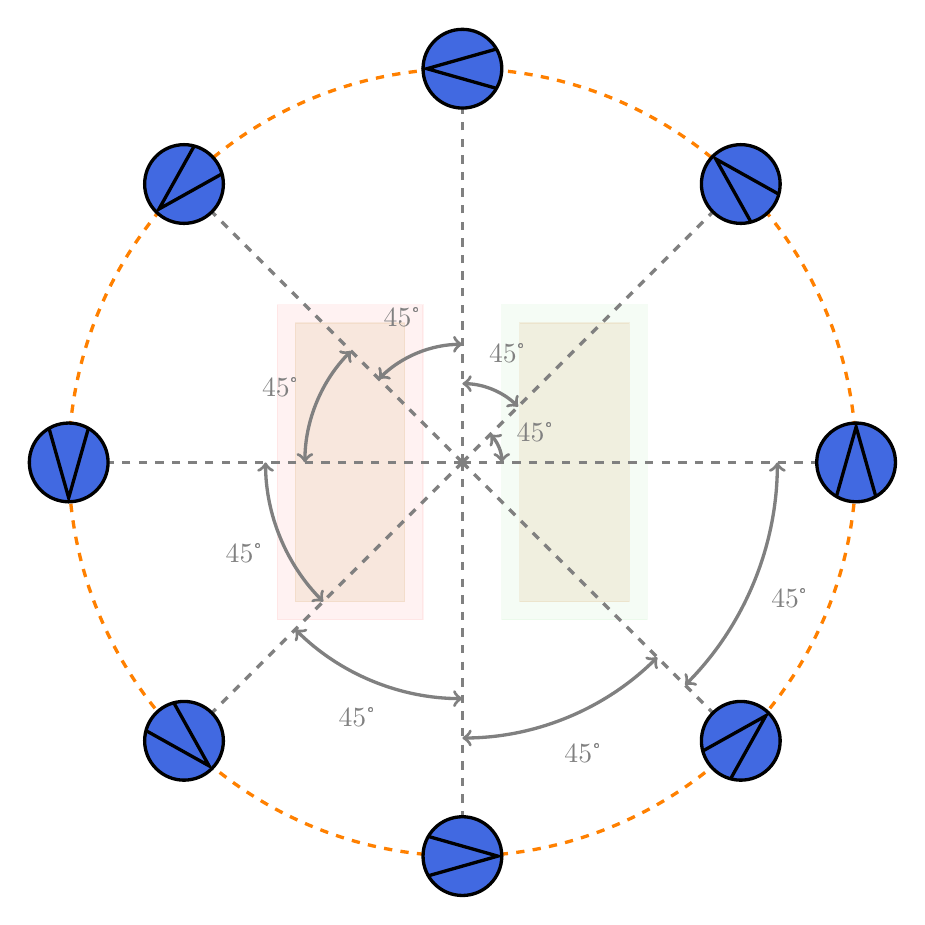
\begin{tikzpicture}

%	\foreach \i in {\xMin,...,\xMax} {
%        \draw [very thin,gray] (\i,\yMin) -- (\i,\yMax)  node [below] at (\i,\yMin) {$\i$};
%    }
%    \foreach \i in {\yMin,...,\yMax} {
%        \draw [very thin,gray] (\xMin,\i) -- (\xMax,\i) node [left] at (\xMin,\i) {$\i$};
%    }

	\draw[red, fill, opacity=0.05] (-0.5,-2) rectangle (-2.35,2);
	\draw[LimeGreen, fill, opacity=0.05] (0.5,-2) rectangle (2.35,2);
	
	\draw[BurlyWood, fill, opacity=0.2] (-0.73,-1.77) rectangle (-2.12,1.77);
	\draw[BurlyWood, fill, opacity=0.2] (0.73,-1.77) rectangle (2.12,1.77);

	\draw[very thick, dashed, orange] (0,0) circle [radius=5cm];
	
	\foreach \i in {0,45,...,315} {
		\draw [very thick, dashed, gray, rotate around={\i:(0,0)}] (0,0) -- (5,0);
		
		\draw [very thick, fill=RoyalBlue, rotate around={\i:(0,0)}] (5,0) circle [radius=0.5];
		\draw [very thick, rotate around={\i:(0,0)}] (5-0.25,-0.433) -- (5,0+0.45) -- (5+0.25,-0.433);
		
		%\draw[rotate around={\i:(0,0)}] (\i*5/360,0) arc [0:30:(\i+45)*4/360];
		\draw [<->, very thick, gray, rotate around={\i:(0,0)}] (\i*4/360+0.5,0) arc [radius=(\i+45)*4/360, start angle=0, end angle=45];
		
		\draw [rotate around={\i+22.5:(0,0)}] (\i*4/360+1,0) node {\textcolor{gray}{45°}};
	}
	
	%\human{0}{0}

	
\end{tikzpicture}
\end{figure}

\end{document}